%---------------------------------------------------------------------------%
\lecture{Research Presentation}{lec_present_conclude}
%---------------------------------------------------------------------------%
\section{\enorcn{Conclusion}{结论}}
%---------------------------------------------------------------------------%
\begin{frame}[fragile]
    \frametitle{Future Work}

    \begin{itemize}
        \item Explore mappings and $\rm{Ra}-\rm{Pr}$ parameter space\newline 

        \item MSTE in different domains: non-cartesian and different aspect ratios\newline 
        
        \item Compute high-$\rm{Ra}$ MSTE using intrinsic $\overline{T}$ profile and $\delta$ scaling
    \end{itemize}
    \begin{columns}[T]
        \begin{column}{.3\textwidth}
            {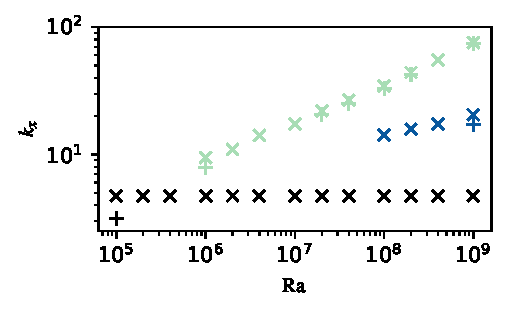
\includegraphics[height=0.75\textwidth]{kx_m_ra1.pdf}}
        \end{column}
        \begin{column}{.3\textwidth}
            {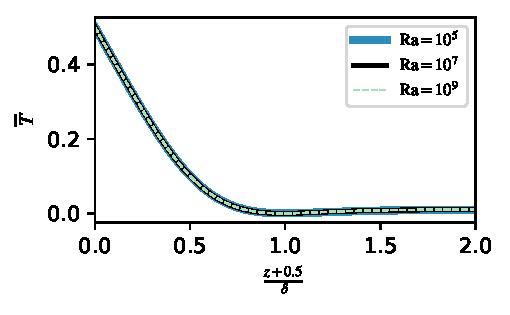
\includegraphics[height=0.75\textwidth]{b0_delta_solid.pdf}}
        \end{column}
    \end{columns}
\end{frame}

\begin{frame}[fragile]
    \frametitle{Acknowledgments}

    \begin{description}
        \item{\textbf{Co-Authors: }} Daniel Lecoanet (Northwestern ESAM), Evan Anders (Northwestern CIERA)\newline
        
        \item{\textbf{Special Thanks: }} Charlie Doering, Baole Wen, Greg Chini, Kyle Augustson, Emma Kaufman, Mallory Drevline\newline

        \item{\textbf{Supported By:}} Northwestern's Walter P. Murphy Fellowship for early career graduate students\newline
    \end{description}
\end{frame}
%%---------------------------------------------------------------------------%
